\section{Alignment process, description of}
\label{app:alignment}

\begin{figure}
\centering
\subfigure{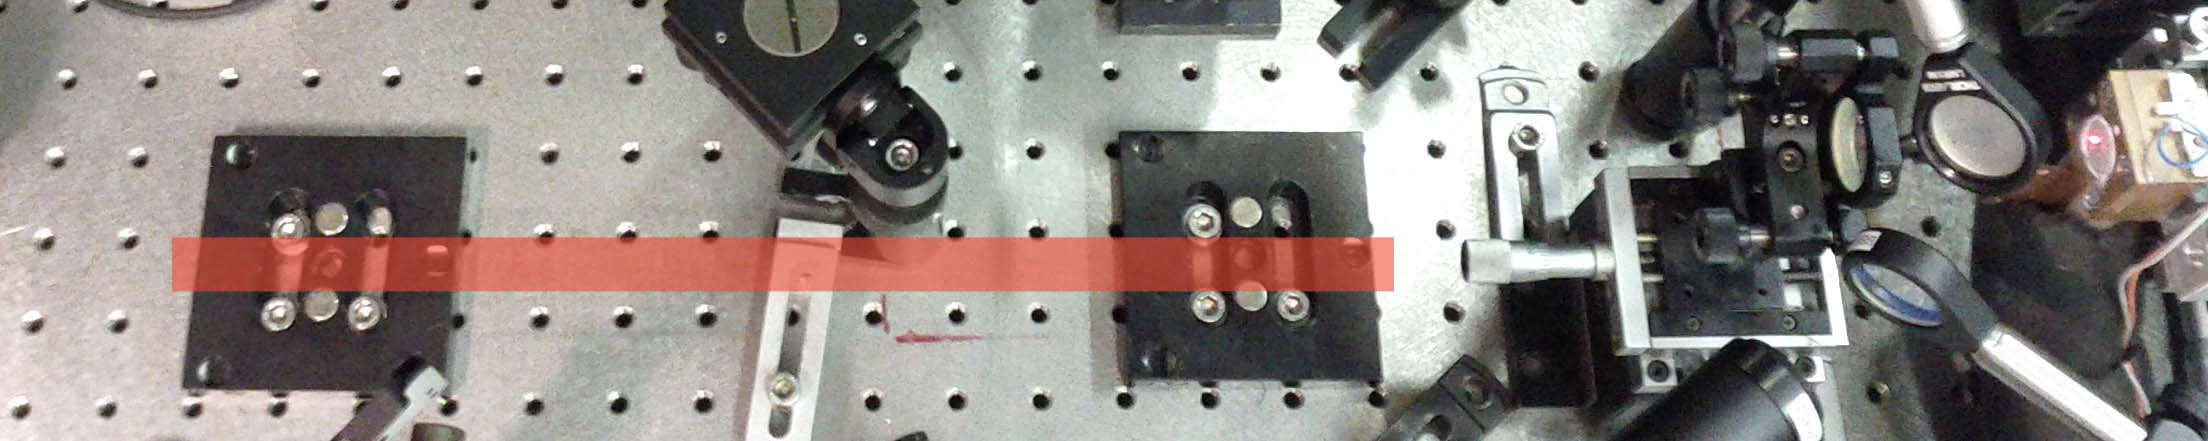
\includegraphics[width=12.5cm]{img/appendix/beamline_empty.jpg}}
\subfigure{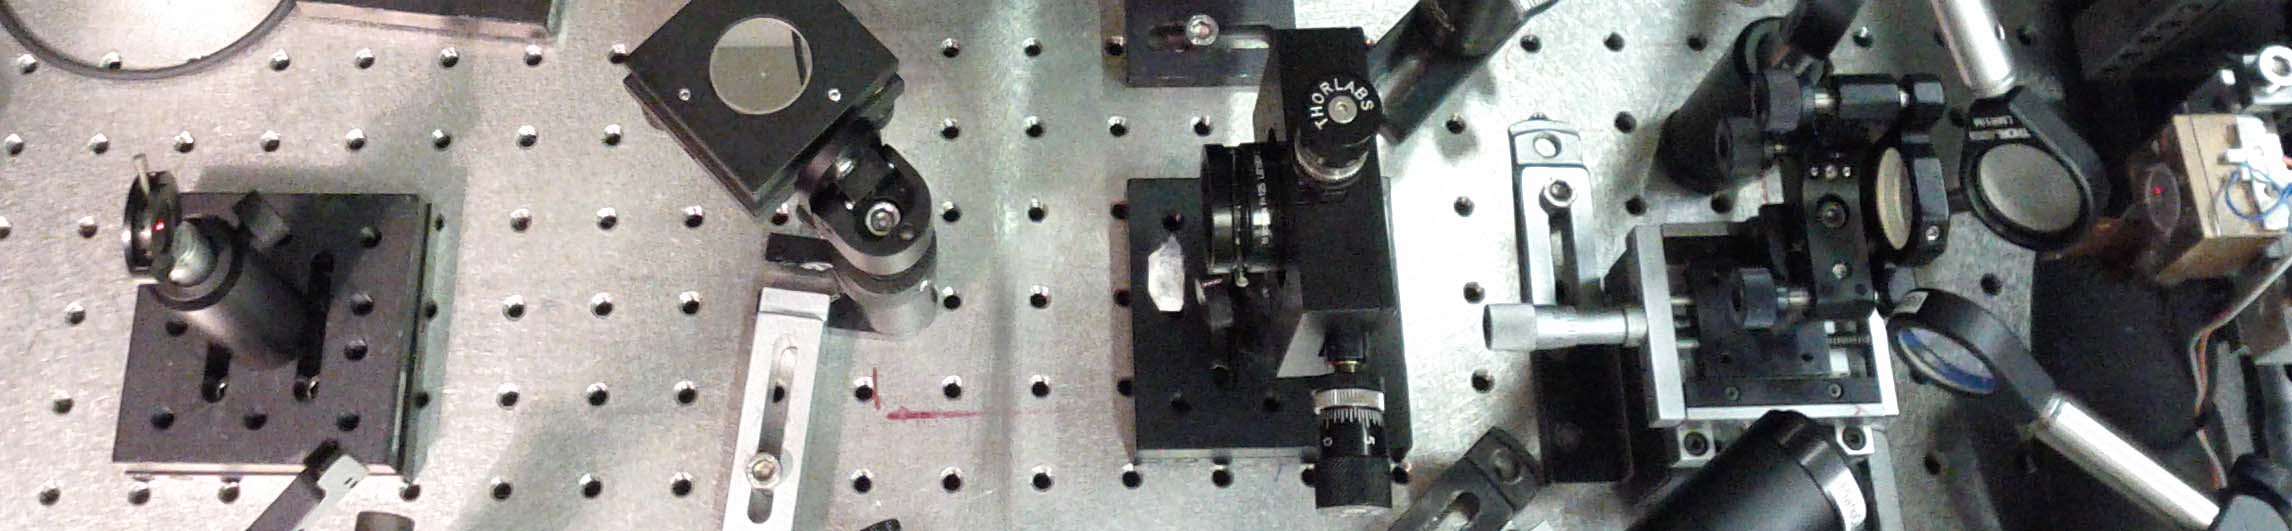
\includegraphics[width=12.5cm]{img/appendix/beamline_populated.jpg}}
\caption{Top: Removeable posts to define the beamline.
Bottom: HeNe beam has to be directed through the two irises.
With these two irises the position of the HeNe source is detached from the beam line.}
\label{img:beamline}
\end{figure}

In order to align the different parts we employ a HeNe laser.
Figure~\ref{img:beamline} shows the beam line orthogonal to the sample surface.
The beam line is defined by two removable magnetic posts.
These posts allow us to remove and replace a mount reproducible.
The beam line is ultimately defined by two irises.
As such, we can place the HeNe source anywhere on the table;
we simply have to guide its beam through these two irises.

For the alignment,
in a first stage,
we align the sample orthogonal to said beam line:
We remove -- or flip, Fig.~\ref{img:cavity_flipped} --
all other components along the beam line
and leave only the sample.
We adjust the orientation of the sample such that
the back-reflection is directed at the HeNe, Fig.~\ref{img:HeNe}.
Once the sample is aligned
we place the output coupler
back in the beam path
and repeat the same procedure.

\begin{figure}
\centering
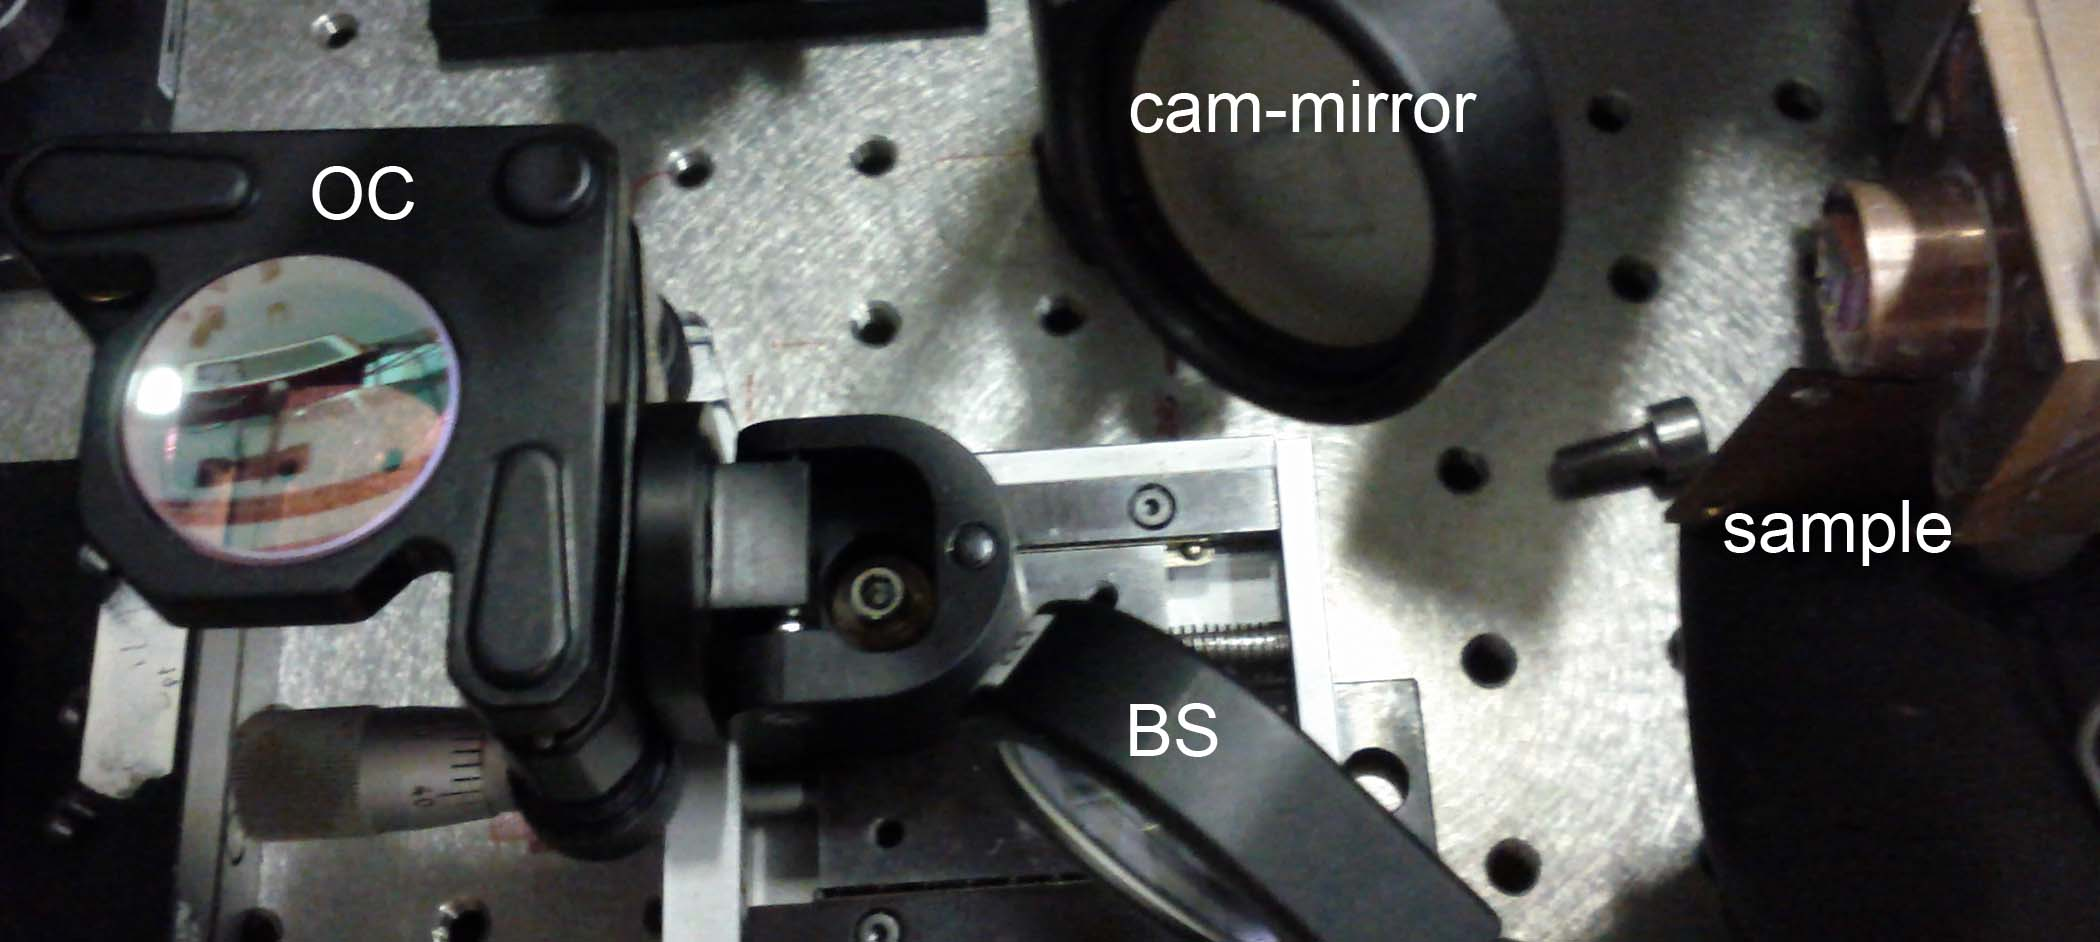
\includegraphics[width=12.5cm]{img/appendix/cavity_flipped.jpg}
\caption{First, we remove / flip all components along the beam line except the sample.
In this configuration we align the sample surface orthogonal to the HeNe.}
\label{img:cavity_flipped}
\end{figure}

\begin{figure}
\centering
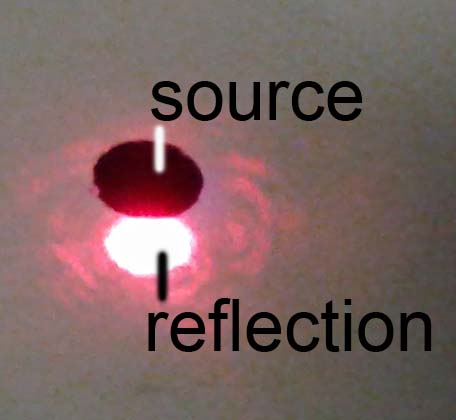
\includegraphics[width=4cm]{img/appendix/HeNe.jpg}
\caption{By arranging the reflected beam to coincide with the HeNe source position
we ensure the orthogonality of the component.}
\label{img:HeNe}
\end{figure}

In a last step we have to irradiate the sample with the 980~nm pump.
A camera along the emission beam line
sees the photoluminescence resulting from the pump on the sample.
This camera is equipped with a long-pass filter
in order to see only the photoluminescence
and not the pump light.
With this camera,
initially,
we see two spots corresponding to
pump and reflection from the output coupler.
Because of the aforementioned alignment with the HeNe laser
these two spots should already be close,
see Fig.~\ref{img:spot_overlap}.
We bring these two spots to overlap,
using the xyz-stage of the output coupler.
Once the two spots do overlap,
and the pump is above threshold,
the sample starts lasing.

\begin{figure}
\centering
\subfigure{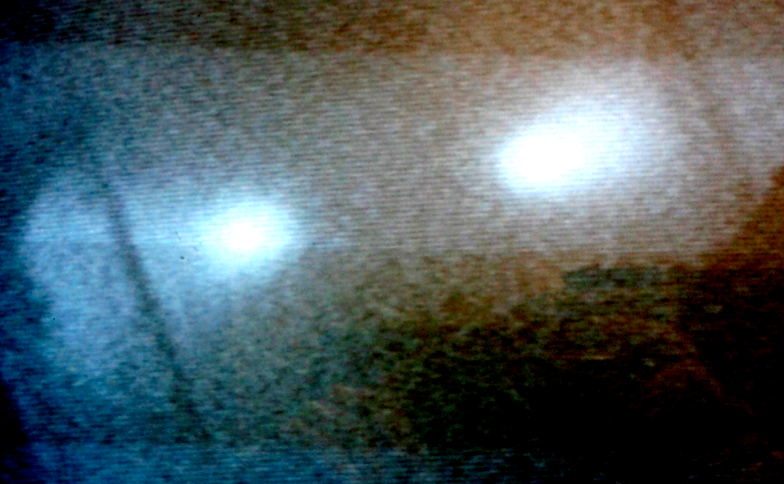
\includegraphics[width=6cm]{img/appendix/spot_overlap_two.png}}
\subfigure{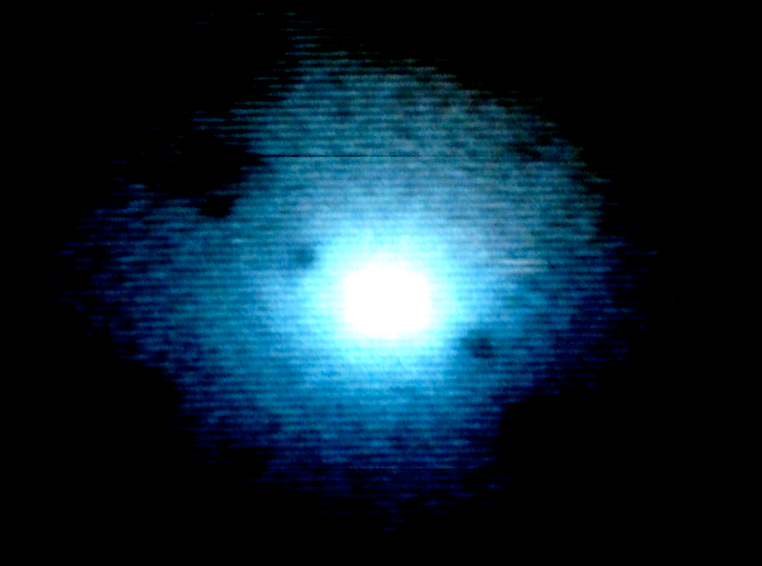
\includegraphics[width=6cm]{img/appendix/spot_overlap_one.png}}
\caption{After the pre-alignment
with the HeNe,
the two spots --
originating
from the pump
and the output coupler reflection --
are close by (left).
By optimizing the alignment
of the output coupler,
these two spots
have to be brought to overlap (right).
Given this configuration,
we have to increase the pump power,
and at threshold we obtain laser emission.
For the fine-alignment
we have to replace the camera
with a power meter
and adjust for maximum output power.}
\label{img:spot_overlap}
\end{figure}

Figure~\ref{img:overview} shows an overview of the different components.
The pump light is directed via fiber to a lens system that images the light onto the sample.
With beam sampler BS$_p$ we extract a fraction of the pump and direct it to detector det$_p$.
This way we have a realtime reading of the pumped power.
A considerable part of the pump light is reflected off the sample.
This light diverges.
First, we thus have to collimate it.
For this we install a lens with appropriate focal length and distance from the sample.
Of this reflected beam we again sample a fraction with BS$_r$,
and direct this to detector det$_r$.
The largest fraction of the reflected beam is directed to the beam dump.
By sampling pump and reflection in this geometry
we avoid high power readings on the detectors.

\begin{figure}
\centering
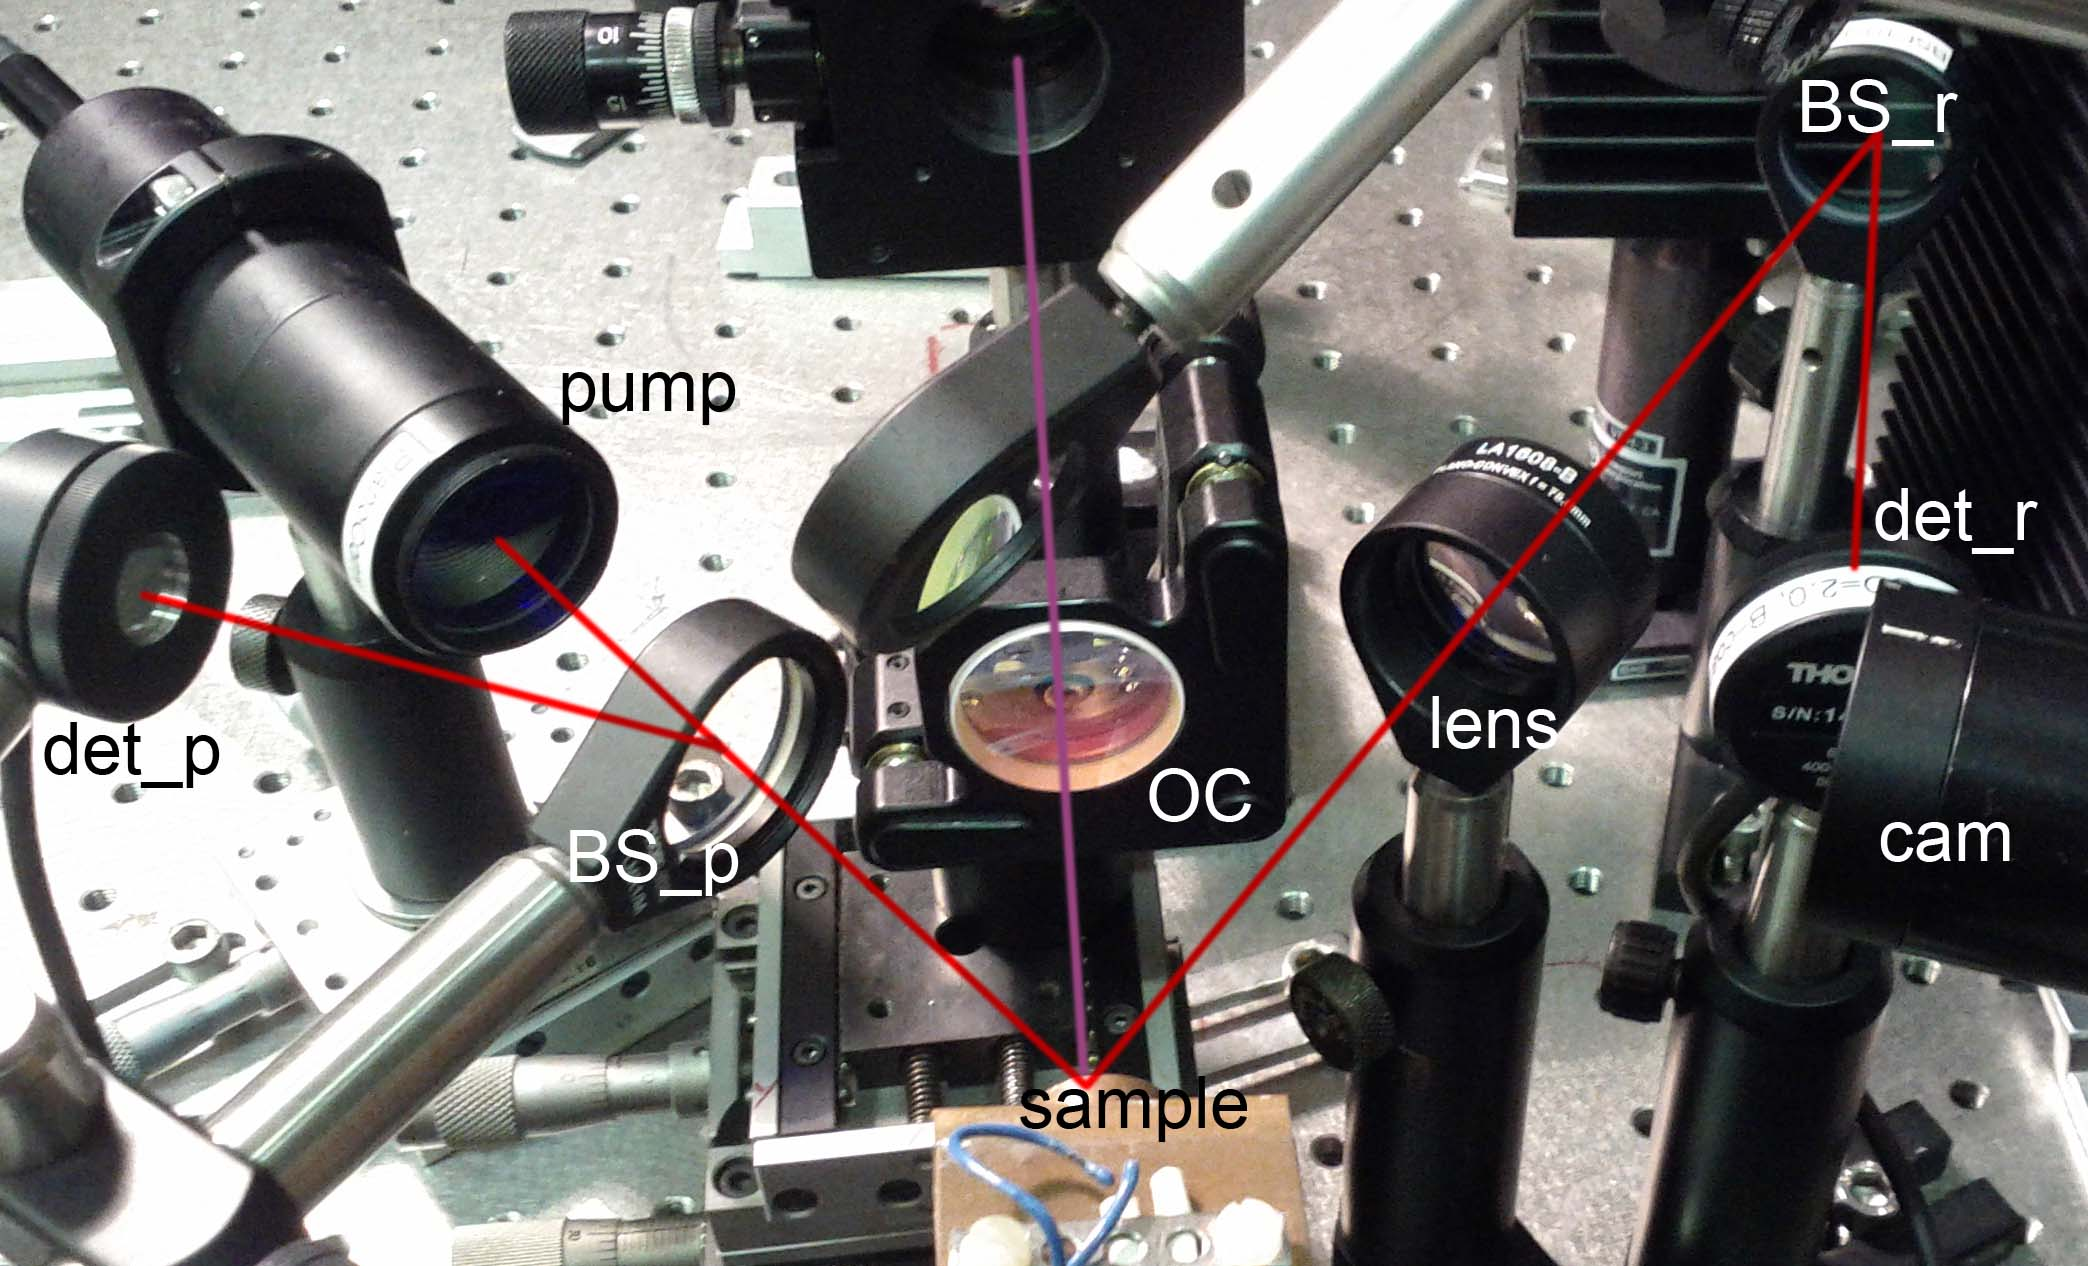
\includegraphics[width=12.5cm]{img/appendix/cavity_all.jpg}
\caption{Overview of the different components incorporated for the cavity.}
\label{img:overview}
\end{figure}




